%
% Angepasste FOM Seminarvorlage
%
\documentclass[12pt,a4paper,listof=totoc,bibliography=totoc]{scrartcl}

\usepackage[english]{babel}			% englische Namen/Umlaute
\usepackage[utf8]{inputenc}	    	% Zeichensatzkodierung
\usepackage{fancyhdr}
\usepackage{graphicx}               % Einbinden von Bildern
% \usepackage[hidelinks]{hyperref}	% Klickbare Verweise und \autoref{label}
\usepackage[colorlinks=true, urlcolor=blue, linkcolor=black, citecolor=black]{hyperref}
\usepackage[intoc]{nomencl}
\usepackage{setspace}
\usepackage{parskip}
\usepackage{caption}
\usepackage{float}
% \usepackage{listings}
\usepackage{geometry}
 \geometry{a4paper, left=40mm, right=20mm, top=40mm, bottom=20mm}
\renewcommand{\familydefault}{\sfdefault}
\renewcommand{\ttdefault}{pcr}
% \renewcommand{\lstlistlistingname}{Listings}
% \renewcommand{\lstlistingname}{Listing}

% Bildueberschrift oben und rechtsbuendig
\captionsetup{labelfont=bf, textfont=bf}
\captionsetup{justification=raggedright,singlelinecheck=false}

% Blocksatz
\def\justify{%
  \rightskip=0pt
  \spaceskip=0pt
  \xspaceskip=0pt
  \relax
}

%
%	Hier werden Titel, Bearbeiter und das Datum eingetragen
%
\newcommand\svthema{Strategies for cookieless online marketing}
\newcommand\svperson{Christian Frank (\#473088)}
\newcommand\svdatum{\today}
\newcommand\lvname{Bachelor-Thesis im Studiengang Wirtschaftsinformatik - Business Information Systems zur Erlangung des Grades eines Bachelor of Science (B.Sc.)}
\newcommand\lvtyp{SS 2021}
\newcommand\lvinst{FOM - Hochschule für Oekonomie \& Management}
\newcommand\lvbetr{Yvonne Romes}

\hypersetup{ % Thema und Author in die Meta-Daten der PDF
  pdftitle={\svthema}, 
  pdfauthor={Christian Frank},
  pdfsubject={Strategies for cookieless online marketing},
  pdfkeywords={Web, Advertising, Marketing, Cookieless}
}

\begin{document}

% Titel
\title{ \huge\textbf{\svthema} }
\author{ {\svperson} \\ \svdatum }
\date{ \normalsize \centering 
\includegraphics[width=0.3\textwidth]{FOM}\\ {\lvname} \\ {\lvbetr} \\ {\lvinst} \\ {\lvtyp} }

% Seitennummer oben
\pagestyle{fancy}
\fancyhf{}
\fancyhf[ch]{\thepage}
\renewcommand\headrulewidth{0pt}

\maketitle
\thispagestyle{empty} % laesst die Seitennummer auf der Titelseite verschwinden
\pagenumbering{Roman}

\begin{abstract}
In this thesis we will evaluate strategies to place meaningful advertisment in a DS-GVO compliant way and without using (tracking) cookies, with an emphasis on technical and legal aspects.

\end{abstract}

\vfill
\begin{figure}[h]
    \centering
    
\includegraphics[]{CC-BY}
\end{figure}

This work is licensed under the Creative Commons Attribution 4.0 International License. To view a copy of this license, visit http://creativecommons.org/licenses/by/4.0/ or send a letter to Creative Commons, PO Box 1866, Mountain View, CA 94042, USA.

\cleardoublepage

\tableofcontents			% Inhaltsverzeichnis
\cleardoublepage

\listoffigures				% Abbildungsverzeichnis
\cleardoublepage

% \lstlistoflistings			% Codeverzeichnis
% \cleardoublepage

%
% Abkuerzungsverzeichnis
%
\makenomenclature
\renewcommand{\nomname}{List of Abbreviations}

\nomenclature{\textbf{APA}}{American Psychological Association}
\nomenclature{\textbf{CCPA}}{California Consumer Privacy Act)}
\nomenclature{\textbf{DMA}}{Digital Markets Act}
\nomenclature{\textbf{DSA}}{Digital Services Act}
\nomenclature{\textbf{DS-GVO}}{Datenschutz-Grundverordnung}
\nomenclature{\textbf{EFF}}{Electronic Frontier Foundation}
\nomenclature{\textbf{EuGH}}{Gerichtshof der Europäischen Union}
\nomenclature{\textbf{FLoC}}{Federated Learning of Cohorts}
\nomenclature{\textbf{GDPR}}{General Data Protection Regulation}
\nomenclature{\textbf{IDFA}}{ID for Advertising}
\nomenclature{\textbf{KPI}}{Key Performance Indicator}
\nomenclature{\textbf{LGPD}}{Lei Geral de Proteção de Dados Pessoais}
\nomenclature{\textbf{NPO}}{Nederlandse Publieke Omroep }
\nomenclature{\textbf{PII}}{Personally Identifiable Information}
\nomenclature{\textbf{POPIA}}{Protection of Personal Information Act}
\nomenclature{\textbf{PPA}}{Privacy Preserving Advertising}
\nomenclature{\textbf{SEO}}{Search Engine Optimization}
\nomenclature{\textbf{SERP}}{Search Engine Result Page}
\nomenclature{\textbf{TTDSG}}{Telekommunikations-Telemedien-Datenschutz-Gesetz}
\nomenclature{\textbf{TÜV}}{Technischer Überwachungsverein}

\printnomenclature[1.5in]          % Abkuerzungsverzeichnis
\cleardoublepage

\pagenumbering{arabic}
\setcounter{page}{5}
\setcounter{secnumdepth}{4}
% \setcounter{tocdepth}{4}

%
%	Einfuehrung
%

\pagebreak
\section{Introduction}

\onehalfspacing

\subsection{Online Marketing and Advertising}

Advertising is the fuel that powers the web. As much as we hate to admit, it's the advertising revenues that fund most of the services available to us on the Internet, from Search to News and Weather. And cat pictures.

The main goal for online marketing and advertising is to increase sales by placing ads that are meaningful to the viewer. To do this, advertising agencies and publishers collect as much data on the viewer as they can, to make sure the advertising is as relevant as possible.

A key technical element in this is the so-called cookie, a piece of information that a website can store on the users' computer, or more precisely, inside the user's browser. These cookies can be evaluated by the site placing them, or by third-parties. With many sites placing cookies and many agencies collecting the data, a complete profile of the user behind the browser emerges and enables the advertising agencies to target their potential customers very precisely.

This type of targeting could not only be used for advertising, but also to exert political influence and affect elections. For the purpose of this paper, we'll focus on the advertising aspect.

The vast amount of data available in user profiles is of concern for privacy experts and several geographies have begun to enact privacy laws, to curb the data collection.

A very contentious point are third-party cookies, which we will analyze in more detail throughout this paper. We will focus on two key aspects, the technical implementation and possible alternatives as well as the legal framework in the European Union for collection such data.

Being able to show meaningful advertising is key for the commercial viability of the advertising business, and thus for the world wide web as a whole. The current changes is tracking cookies will have a big effect on the industry and we want to use this paper to gain some insights and develop strategies going forward.

The overall situation is still very much in flux and there is no clear consensus on a way forward; very recently Google has announced to extend the life of third-party cookies until the end of 2023.\footnote{See \textit{Goel, V. (2021)}: An updated timeline for Privacy Sandbox milestones. \cite{sandboxDelay}}

In this paper I will focus on the current state at the time of writing and rely on expert opinions from the field of online marketing.

\subsection{Gender-neutral Pronouns}

Our society is becoming more open, inclusive, and gender-fluid, and now I think it's time to think about using gender-neutral pronouns in scientific texts, too. Two well-known researchers, Abigail C. Saguy and Juliet A. Williams, both from UCLA, propose to use singular they/them instead: "The universal singular they is inclusive of people who identify as male, female or nonbinary."\footnote{\textit{Saguy, A. (2020)}: Why We Should All Use They/Them Pronouns. \cite{pronouns}} The aim is to support an inclusive approach in science through gender-neutral language. 

In this paper, I'll attempt to follow this suggestion and invite all my readers to do the same for future articles. Thank you!

If you're not sure about the definitions of gender and sex and how to use them, have a look at the definitions\footnote{See \textit{APA (2021)}: Definitions Related to Sexual Orientation. \cite{apaDefinitions}} by the American Psychological Association.

Also, to be mindful in our writing, requires careful evaluation of the terminology we use in our text and a certain level of restraint. For this paper, I use a handy reference to ableist terms\footnote{See \textit{Brown, L.X.Z. (2021)}: Ableism/Language. \cite{ableismLanguage}} that I want to avoid.

\subsection{Tools}

I wrote the LaTeX \href{https://github.com/chfrank-cgn/Bachelor-Arbeit}{source code} for this thesis with \href{https://www.overleaf.com/}{Overleaf} as the main editing tool and \href{https://github.com/}{GitHub} for revision control, I checked for grammar, style, and plagiarism with \href{https://app.grammarly.com/}{Grammarly}, and I had \href{https://www.youtube.com/watch?v=5qap5aO4i9A}{LofiGirl} for the soundtrack of my writing.

\subsection{Acknowledgments}

I am very grateful to \href{https://www.linkedin.com/in/yvonne-romes/}{Yvonne Romes}, lecturer at FOM, for their support on this thesis; I am extremely thankful and indebted to them for sharing expertise, and sincere and valuable guidance and encouragement extended to me.

I am also very grateful to the members of my expert panel, without their generous and patient support this paper would not have been possible.


%
%	Begrifflichkeiten
%

\pagebreak
\section{Targeting Background}

\onehalfspacing

\subsection{Targeted Advertising}

\subsubsection{Rationale}

Why do we need targeted advertising?

Let's start with the basics: Any advertising or marketing business has a vested interest to make their ads relevant, especially on the world wide web, where the user is, at least to a certain extent, anonymous. In its very basic, offline form, agencies would use context to place their ads; as an example you might see advertising for cars on busy roads or advertising for food near supermarkets.

In the online world, targeting users can be much more granular and automated, with the ideal outcome of showing an ad exactly at the right time and the right place (e.g. web site) for the user to see it, and with a need that it fulfills, have the user buy the product.

Showing personalized advertisement by targeting the right user at the right time is important for established as well as new market entrants.

In a recent report, \href{https://www2.deloitte.com/de/de.html}{Deloitte} found that 74\% of small businesses using personalized ads stated that they were important for the success of their business.\footnote{\textit{Deloitte LLP (2021)}: Dynamic Markets \cite{deloitteSmb}} 68\% of the surveyed small companies said that the use of personalized, targeted advertising helped them to achieve a higher return on their marketing spend.

To achieve this, and show personalized and targeted advertising, ad placement uses micro-targeting on the world wide web.

"Microtargeting is a marketing strategy that uses people’s data — about what they like, who they’re connected to, what their demographics are, what they’ve purchased, and more — to segment them into small groups for content targeting. It’s the reason that if you typically shop at Whole Foods, you may be served an advertisement for organic sunscreen during the Summer. And while it can help deliver content that is interesting and helpful to you, it also has a dark side — especially if it delivers information that’s inaccurate or biased and meant to sway your vote."\footnote{\textit{Ghosh, D. (2018)}: What is microtargeting? \cite{mozillaBlog}}

From a business point of view, showing persoanlized ads through micro targeting dramatically increases the relevance of the shown advertising and thus the likelihood of the user noticing it. Even if it does not lead to a sale right away, any product awareness helps and might lead to a sale in the future. 

Give the automated nature of ad placement on web pages, there is no longer a need for ads to be shown in bulk, like in the offline world, but can be shown individually and with high relevance. 

\subsubsection{Tracking}

To achieve this, it is necessary to gather more information on the interests of a particular user and follow their interests across the web; this mechanism is called tracking. Tracking as of today heavily relies on the use of cookies, small pieces of information stored in the users' browser, which we will explain in the next section.

Tracking can span web sites and companies - it is not limited to one company keeping a record of ones visits, currently it also includes the ability to analyze all visits on cooperating pages and show, for example, ads on Facebook based on your recent queries at Amazon. Technically this can be achieved through third-party cookies.

Third-party cookies are cookies set by another website than the one you're currently visiting and that can be later evaluated from the website.\footnote{See \textit{Cookie Script (2021)}: All you need to know about Third-Party Cookies \cite{mozillaBlog}}

Tracking through third-party cookies is under attack from multiple angles;\footnote{See \textit{Brinkmann, M. (2021)}: How Firefox new SmartBlock feature works \cite{mozillaBlog}} even \href{https://www.google.com/}{Google}, who invented it among various other tracking methods, will no longer support it in \href{https://www.google.com/chrome/}{Chrome} after 2023.\footnote{See \textit{Goel, V. (2021)}: An updated timeline for Privacy Sandbox milestones. \cite{sandboxDelay}}

Placing targeted ads currently makes heavy use of tracking, especially in the form of tracking cookies, however, it can also make use of publicly available information, such as social media posts, as we will see later in this paper.

\subsubsection{Cookies}

Let's go back to cookies and have a look at what it is.

A cookie is a small piece of information that a server sends to the user's web browser for storage, and which it can request back at a later point in time.

Cookies can be used for session management, personalizing and tracking.\footnote{See \textit{Mozilla (2021)}: Using HTTP cookies \cite{usingCookies}} For the purpose of this paper, we will focus solely on the tracking aspect, especially across sites, and do not cover the more benign use cases for cookies, such as session management, in any detail.

From this explanation we can see that cookies in itself are not malign and greatly support the user's experience across the web. However, they also include a persistent history of the user's activities which can be used to track the users' journey across the web.

Let's have a look at where cookies live on a user's browser. As an example, we will look at \href{https://www.mozilla.org/en-US/firefox/new/}{Firefox}, which stores its cookies in a \href{https://www.sqlite.org/index.html}{SQLite} database in the user's profile directory. Using \href{https://sqlitebrowser.org/}{DB Browser for SQLite}, we can have a look at the cookies on our computer:

\begin{figure}[H]
\centering
\caption {Cookie Details in Firefox}
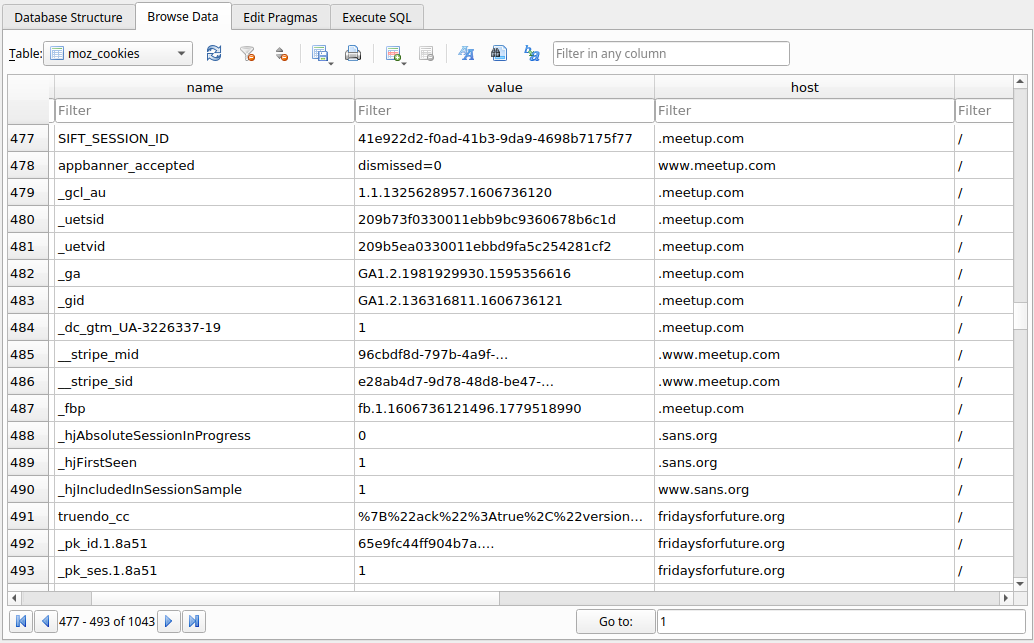
\includegraphics[width=\linewidth]{images/cookie-sqlite.png}
\label{fig:cookies}
\end{figure}

In its technical essence, cookies are a simple key-value store in the browser, that stores its data per host, or more precisely, per web site. It's entirely up to the web site to define which keys it wants to store and which values it wants to set and thus persist across visits. 

If a web site accesses it's own cookies (as defined in the hosts column), that's called a first party cookies and it's part of first party data. This could be used for session persistence, for example, as seen in the first column. We'll define these data types in the next chapter.

If a web site accesses data from another site, that's when we're talking about referencing third party cookies as part of third-party data. Data from other web site's cookies could be used to track users on their visits across different web sites and has become a big privacy concern over the last couple of years. This tracking aspect across sites is what primarily motivates this paper.

In addition to tracking in the web browser, there's also tracking in E-Mail\footnote{See \textit{Doffmann, Z. (2021)}: Why You Suddenly Need To Delete Gmail On Your iPhone \cite{deleteGmail}}, however, we will not cover E-Mail tracking in this paper.

\subsection{Data Types}

\subsubsection{First Party}

Now that we have covered cookies as a mechanism to persist data in the user's browser across sessions, we need to look at the various classes of data, define their usage and prepare for the analysis of their relevance in regards to privacy regulations.

The definition for first party data is actually quite simple, it is data that we collect from our own sources.\footnote{See \textit{OnAudience (2019)}: What is first party data? \cite{firstParty}} Data could include information that we retrieve from our own cookies or from any information the user might have left on our website, for example by looking at an item. It also includes registration information, shop logins and past sales or other interaction. Collection this kind of data is not a big issue from a privacy point of view, as long as it's done correctly and with the necessary precautions against abuse in place.

As an example, in a web shop, a clever use case for using ones own shop data for marketing would be to follow up on an abandoned sale, where the user looked at an item but did not put it into their shopping cart:

\begin{figure}[H]
\centering
\caption {Zumiez Follow-Up EMail}
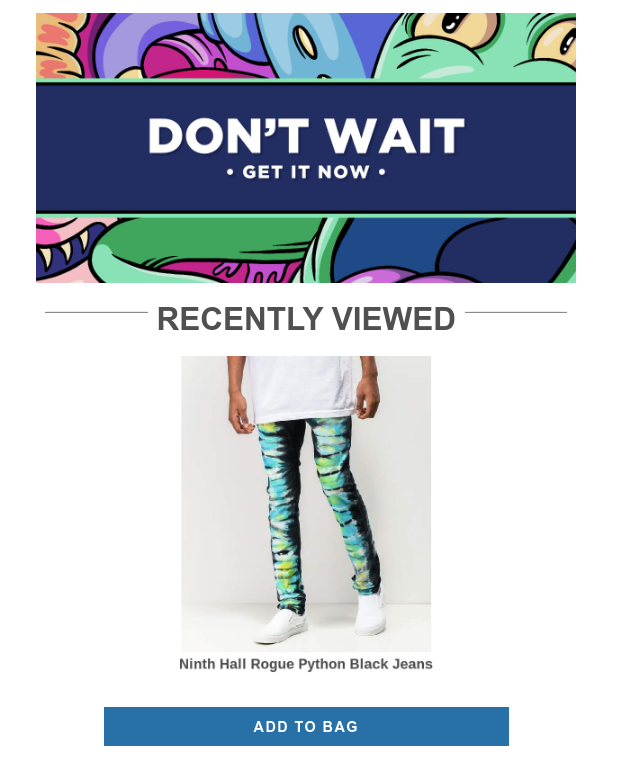
\includegraphics[scale=0.6]{images/zumiez-dont-wait.png}
\label{fig:zumiez}
\end{figure}

This screenshot was taken from an E-Mail by \href{https://www.zumiez.com/}{Zumiez}, prompting the user to follow through with buying an item that they looked at the day before.

Another example of clever use of first-party data for marketing are the regular notifications from \href{https://www.netflix.com/de-en/}{Netflix} to finish the season of a series you just started, or, as we will see further below, the advertising \href{https://smile.amazon.de/}{Amazon} places on its own web pages.

% \begin{figure}[H]
% \centering
% \caption {Continue Watching}
% 
\includegraphics[width=\linewidth]{images/continue-boruto.png}
% \label{fig:boruto}
% \end{figure}

\subsubsection{Second Party}

The second class of data that we will look at is second party data. Simply speaking, second party data is another companies first party data.\footnote{See \textit{OnAudience (2019)}: What is first party data? \cite{firstParty}}

Assuming that two companies use the same identifier for their customers, for example the E-Mail address, one company could sell the shopping history on their site to another company, to enable them to advertise related products. Another option would be to not sell the data outright but to establish a cooperation and use the data from both parties across both web sites.

As we will see later in this paper, from a legal perspective, this is the most difficult setup to achieve. Both companies would need explicit consent from all its users to transfer their data to the other company, they would otherwise open themselves up for a lot of legal trouble and violate the trust and privacy of their customers.

It can be achieved though, for example within a conglomerate such as \href{https://www.facebook.com/}{Facebook}, \href{https://www.whatsapp.com/}{WhatsApp} and \href{https://www.instagram.com/}{Instagram}, where platform users are explicitly asked to allow their data to be shared across all platforms. In case of WhatsApp, the announcement to cooperate on user profiles with the parent company in the short term led to ab exodus of some users that greatly benefited the competing platforms. In the long term, however, the integration did go well and the users now experience a streamlined profile management and smooth interoperability. Monthly WhatsApp users in July of this year now exceed 2 billion and numbers are growing steadily.\footnote{See \textit{Statista (2021)}: Most popular global mobile messenger apps \cite{whatsStats}}

In summary, we can conclude that if the proper agreements with the users are in place and the sharing is transparent, the use of second party data can be beneficial to both consumers and providers, and can greatly enhance the shopping experience for all involved parties.\footnote{See \textit{Schneier, M.J. (2017)}: Protecting customer privacy when marketing with second-party data \cite{secondParty}}

\subsubsection{Third Party}

The last class of data we want to look at is third party data. It's defined as additional data that you buy from specialized sources on the web to enrich your own data.\footnote{See \textit{OnAudience (2019)}: What is first party data? \cite{firstParty}}

Third party data can be derived through the use of third party cookies. As the user travels the web and leaves their traces in the cookies of their browser, data management platforms harvest this information, anonymize it, and create profiles from it.\footnote{See \textit{Shiffman, E. (2020)}: What is Third-Party Data? \cite{thirdParty}} These profiles are then sold and can be used to enrich ones own data.\footnote{See \textit{Sponder, M. (2017)}: Digital Analytics for Marketing - Understanding and Working with Third-Party Data \cite{digitalAnalytics}}

Other sources of third party profile information is the data that users leave voluntarily on the web, such as in their public social media profiles and posts, or location information from their fitness trackers.

With the impending demise of the tracking cookie, some aspects of the harvesting of third party data might go away and user profiles might become less readily available on the web to purchase, or otherwise available for targeted advertising.

As we progress in the paper, we will try to identify other strategies to display meaningful advertisement without using the data obtained from tracking cookies.

\subsection{Toolstack - Analytics}

\subsubsection{Google Analytics}

To be able to judge whether out advertising is meaningful and successfully placed, we need to analyze the traffic to our page and the behavior of our users.

Let's first look at the tools that allow us to analyze traffic to our site and evaluate key performance indicators for our campaigns, such as Click-Through or Conversion rates.\footnote{See \textit{Romes, Y. (2020)}: 10 Inbound KPIs, die jetzt auch Personaler kennen sollten \cite{inboundKPI}}

\href{https://analytics.google.com/}{Google Analytics} is the most widely used tool for web traffic analysis and gives us, according to its website, all the necessary tools to analyze your web business data and gain insights into your campaign performances.

By looking at the data provided, we can gather deep insights into the visitors of our page and predict the performance of our posts.\footnote{See \textit{Frank, C. (2021)}: Web Traffic Analysis - Predicting Blog Post Performance \cite{previousBigdata}} We can also measure the effectiveness of our ad campaigns, which is another and very different topic, and out of scope for this paper.

\subsubsection{Open Source Analytics}

In addition to Google Analytics, there are a couple of other alternatives, some of which are \href{https://opensource.org/osd}{open source}. One example for open source analytics is \href{https://plausible.io/}{Plausible}, which I covered in a previous paper and which claims to be fully compliant to all major privacy legislation.\footnote{See \textit{Frank, C. (2020)}: Usefulness of open-source tools for web analytics in EMarketing \cite{previousPaper}} 

For the scope of this paper, we will from here on only focus on the data sources that we can use to place our campaigns, and not on the metrics that are needed to support our campaigns.

However, to illustrate, here's a view of a main web analytics dashboard:

\begin{figure}[H]
\centering
\caption {Plausible Web Analytics Dashboard}
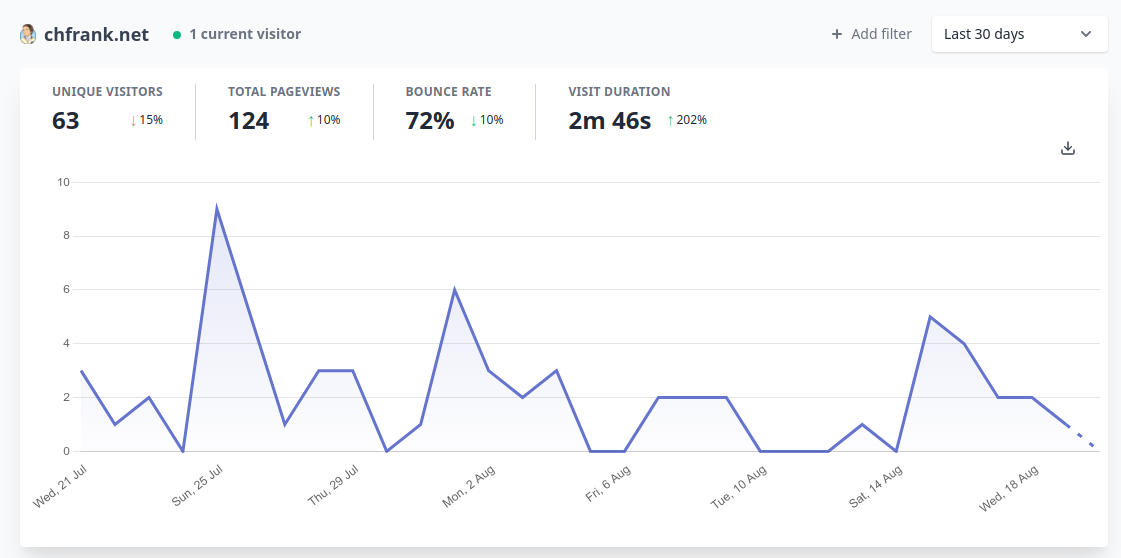
\includegraphics[width=\linewidth]{images/plausible.png}
\label{fig:plausible}
\end{figure}

\subsubsection{Yandex Metrica}

If you're reluctant to send data to the US for processing but are at the same time not invested in the open source side of software, \href{https://metrica.yandex.com/}{Yandex Metrica} is another commercial option for web page analytics, covering more than 8 million sites, according to their web page.

Metrica is part of the Yandex family of tools; Yandex is headquartered in Moscow, Russia and operates the biggest search engine there.

Yandex Metrica and Google Analytics are both operated by major search engine providers, which is not that surprising - in addition to crawling the web these search engines need to perform a lot of analytics themselves to put the most relevant search results on the first page. It makes a lot of sense to expose these analytics in some form to the end users.

How to optimize your placement on the search engine result page, is a wholly different topic which we again will not cover in this paper.

\subsection{Toolstack - Advertising}

\subsubsection{Google Ads}

Now that we have identified the data sources for successful advertising campaigns and the tools to measure the success, we need to look at the platforms that we could place our campaigns on. 

The biggest platform is \href{https://ads.google.com/home/}{Google Ads} and you can use it run campaigns on Google's search engine result pages and affiliates.

Ad placement on Google is based on search keywords and Google's knowledge of the user's profile; Google operate a bidding website where you place bids for certain terms and demographics to get your particular ad shown. Ad placement and the underlying algorithm is a science unto itself; recently Google has come under scrutiny from the regulators and in one case, agreed to the ruling and the fine.\footnote{See \textit{Burgess, M. (2021)}: France Cracked Down on Google’s Ad Tech \cite{googleAds}}

To target the most appropriate users for an ad, Google needs to have accurate information on the user itself and that's where third party data and data from third party cookies comes in.

It's important to differentiate between ad placement, which is a paid-for service, and search engine result page placement, which can be improved through Search Engine Optimization (SEO) techniques - even though both techniques are related to the Google search engine, they are not the same.

\subsubsection{Amazon Advertising}

The second biggest advertising platform is \href{https://advertising.amazon.com//}{Amazon Advertising}, a platform to place ads for your products on Amazon's pages and their affiliates.

The biggest difference to Google Ads is in that Amazon Advertising already has all the relevant data from their users through the Amazon shopping web site. Amazon Advertising can almost operate entirely with its own first party data. It has user preferences, shopping history and recent searches, all from its own data source and obtained with full consent from its users

Amazon Advertising also operates as a demand-side platform with selected partners, to increase the reach of the ads placed, which would be a case of cooperation and the use of second party data.

With ads focused on the Amazon shopping experience and consent from their users obtained on sign-up, Amazon's advertising business is not that much affected by the current discussion about third-party data.

\subsubsection{Facebook Advertising}

Last but not least we need to mention \href{https://www.facebook.com/business/ads}{Facebook Ads}, a platform to place ads on Facebook, Instagram, Messenger and the Audience Network.

Similar to Amazon, Facebook already has all the user profile data that it needs from its own platforms and has obtained consent during sign-up to share that data within its own family of businesses.\footnote{See \textit{WhatsApp (2021)}: What information does WhatsApp share with the Facebook Companies? \cite{whatsApp}}

Both companies, Amazon and Facebook, sit on a vast trove of invaluable first and second party data that they can freely use for their advertising business, without needing to resort to third party data.

Knowing this, Facebook is currently running an extensive campaign in the moment to recruit new business customers for their personalized advertising offering.\footnote{See \textit{Facebook (2021)}: Dein Unternehmen ist es wert, entdeckt zu werden \cite{facebookAds}}

\subsection{Moving past cookies}

\subsubsection{Browser-based}

To continue with targeted advertising, even after the demise of the tracking cookie, new concepts and data sources are needed, some of which we will present and analyze in this paper with the goal to develop possible strategies for online marketing going forward.

A common thread of all the new approaches is the attempt to make targeted advertising work, while at the same time maintaining the user's privacy; an umbrella term for these approaches is Privacy Preserving Advertising.\footnote{See \textit{Rescorla, E. (2021)}: The future of ads and privacy \cite{futureAds}}

The primary contender in the PPA space is \href{https://wicg.github.io/floc/}{Google FLoC}. The idea behind the Google's federated learning of cohorts is actually quite simple, as it aims to expose the users' general browsing interest without exposing the browsing history, as it is the case today through the widespread use of third party cookies.

To achieve this, Google proposes an algorithm to assign cohort ids to individual browsers, based on shared browsing habits. Then, instead of placing ads towards personally identifiable user profile data, ads would be placed against an anonymous cohort. 

The idea behind FLoC itself sounds quite reasonable, it is, however, under heavy fire from a privacy point of view.\footnote{See \textit{Rescorla, E. (2021)}: Privacy analysis of FLoC \cite{privacyFloc}} Among others, \href{https://www.eff.org/}{EFF}\footnote{Disclosure: I am a member and active supporter of EFF} has published a detailed analysis of FLoC's shortcomings in regards to privacy and why they believe that FLoC would be a terrible idea.\footnote{See \textit{Cyphers, B. (2021)}: Google’s FLoC Is a Terrible Idea \cite{terribleIdea}}

One of the biggest concern is that by combining the FLoC data with browser fingerprinting, for example, super profiles could be created that would contain much more information than is available today. In summary, all currently available analysis question the actual ability of FLoC to maintain the user's privacy and foresee a much broader tracking of users and their profiles than currently through the use of third party cookies.

It is worth to note that the issues with FLoC center around privacy, not the algorithm itself - federarted learning is a well establish technique in the field of machine learning.\footnote{See \textit{Li, T. (2020)}: Federated Learning: Challenges, Methods, and Future Directions \cite{9084352}}

\subsubsection{Identity-based}

Similar to FLoC are several other approaches that implement some kind of advertising ID instead, which would attempt not to violate the user's privacy rights and still allow for targeted advertising. 

The most prominent approach was Apple's ID for Advertising, which does not seem to be going anywhere for the time being.\footnote{See \textit{Ray, O. (2020)}: What is IDFA and Why Apple Killed it \cite{cleanRoom}}

Google also has an Advertising ID that supports ad personalization based on preference.\footnote{See \textit{Google (2021)}: Advertising ID \cite{advertisingId}} Similar to Apple's ID, Google offers an opt-out mechanism; if you opt out, only generic ads will be shown with much less relevance, and with a much lower chance of a sale for the company placing the ad.

An industry consortium is releasing an open-source ID standard, UID2.\footnote{See \textit{The Trade Desk (2021)}: Unified ID Soltution 2.0 \cite{tradeDesk}} The basic premise is the same as for Google's or Apple's ID - the user is identified through a piece of personal information that is then encrypted and used as ID for the advertising profile. Unlike the approach from Apple and Google, however, the ID is not based on the device or the browser, but would require an active login. Quite elegantly this would solve all issues around consent and privacy, but it remains to be seen how many users will be logging in to an advertising network and share their preferences, just to get better ads displayed.

Also, Microsoft is working together with the Harvard University on yet another standard\footnote{See \textit{Bird, S. (2020)}: Introducing the new differential privacy platform \cite{openDp}}, \href{https://opendp.org/}{OpenDP}, based on Differential Privacy.\footnote{See \textit{OpenDP (2020)}: What is Differential Privacy? \cite{diffPrivacy}} The conceptual idea behind differential privacy is quite interesting, but an analysis is out of scope for this paper.

\subsubsection{Data-based}

A completely different option would be to do away with third party data altogether and focus solely on second party data to augment ones own data. 

One way to achieve this could be through data clean rooms, where independent contract processors would anonymously combine first party data of two or more companies and return the aggregated results to all parties. Having independent data trustees that vouch for anonymity could make sure that such data processing would not run afoul of data protection regulations.\footnote{See \textit{Younger, M. (2019)}: The Three Hidden Technology Trends Behind Data Clean Rooms \cite{cleanRoom}}

Even though this approach sounds quite promising, such an independent infrastructure does not yet exist and no supra-national body has stepped up to create it.

\subsubsection{Content-based targeting}

Another quite interesting approach is to forfeit user-based targeting altogether and concentrate solely on the browsing context. In 2020, the public radio in The Netherlands did this and went from targeted advertising to contextual advertising; quite surprisingly they saw their ad revenues grow.\footnote{See \textit{Edelman, G. (2020)}: Can Killing Cookies Save Journalism? \cite{killingCookies}} 

The system at \href{https://over.npo.nl/}{NPO} is a bidding system similar to Google Ads, however, ads are not placed based on a user profile but on the current context, i.e. a web page shown or a TV show watched. As far as the documentation shows, there's never any personally identifiable information being collected or transmitted and thus no issue at all with violating the user's privacy.

Abandoning the user profile in favor of context feels a bit like going back in time, but it does eliminate all privacy woes.

\subsection{Legal Framework}

As the final chapter of this section, we need to have a brief look at the privacy laws and regulations that have come up in recent times. 

With privacy coming into more and more focus, legislation is being drafted all over the world to better protect the user's privacy, eliminate unauthorized data collection and fight surveillance capitalism.\footnote{See \textit{Zuboff, S. (2020)}: You Are Now Remotely Controlled \cite{surveillance}} 

There's quite a number of legal frameworks that begin to govern tracking and advertising, so here's a list of the most common ones with links to the respective legal texts:

\begin{itemize}
 \item \href{https://gdpr-info.eu/}{GDPR} (General Data Protection Regulation)
 \item \href{https://www.datenschutz-grundverordnung.eu/}{DS-GVO} (Datenschutzgrundverordnung)
 \item \href{https://dsgvo-gesetz.de/bdsg/}{BDSG} (Bundesdateschutzgesetz)
 \item \href{https://dsgvo-gesetz.de/ttdsg/}{TTDSG} (Telekommunikations-Telemedien-Datenschutz-Gesetz (Entwurf ))
 \item \href{https://oag.ca.gov/privacy/ccpa}{CCPA} (California Consumer Privacy Act)
 \item \href{https://www.lgpdbrasil.com.br/}{LGPD} (Lei Geral de Proteção de Dados Pessoais)
 \item \href{https://popia.co.za/}{POPIA} (Protection of Personal Information Act)
 \item \href{https://ec.europa.eu/info/strategy/priorities-2019-2024/europe-fit-digital-age/digital-services-act-ensuring-safe-and-accountable-online-environment_en}{DSA} (Digital Services Act)
 \item \href{https://ec.europa.eu/info/strategy/priorities-2019-2024/europe-fit-digital-age/digital-markets-act-ensuring-fair-and-open-digital-markets_en}{DMA} (Digital Markets Act)
\end{itemize}

We cannot dive into the details on all these regulations; for the purpose this paper, we will assume that the reader is familiar with the content of the most important ones for Europe and Germany, the GDPR/DS-GVO and the BDSG, and will from here on solely focus on their impact and interpretation.

We've covered all basic aspects of tracking and targeting and introduced the most relevant tools and current developments. To continue to come up with strategies for online marketing beyond the end of the tracking cookie, it's now time to bring in the experts.


%
%	Theorieteil
%

\pagebreak
\section{Research Methodology}

\onehalfspacing

\subsection{Developing Situation}

The current situation in regards to targeting and tracking cookies as enabling technology is under heavy development and undergoing changes almost on a daily basis; for this paper we will look at developments up until the end of July 2021 and hope that by the time you read this it will still be somewhat relevant.

Literature is still sparse, and thorough quantitative analysis has yet to be done. To deliver the most value and reach an answer to our research question on which strategies we can develop to place meaningful advertisement in the future, in a DS-GVO compliant way and without using cookies, we're choosing a qualitative research method.

We want to place an emphasis on technical and legal aspects and hence will focus our research on these aspects and aim to reach a conclusion at the end of our analysis.

\subsection{Content Analysis}

The most fitting method for the research at hand is Qualitative Content Analysis as pioneered by Philipp Mayring, who developed a framework to perform structured qualitative analysis of text through content analysis.\footnote{See \textit{Mayring, P. (2020)}: Qualitative Content Analysis \cite{qualiContent}} During his tenure at the university of Klagenfurt, Phillip Mayring defined a stringent procedural approach on how to analyze text and deduct research information from it, using inductive development of categories and subsequently the deductive application of these.

\subsection{Expert Interview}

Rather than analyzing the myriads of available opinion texts on the web, we decided to use a panel of experts, to gather the most up-to-date expert knowledge and provide the most value. Our approach of conducting expert interviews is based on Robert Kaiser's book on the same topic.\footnote{See \textit{Kaiser, R. (2014)}: Qualitative Experteninterviews \cite{expertInterviews}}

Especially since there is not yet an established field of expertise and literature on this topic available, using an expert panel seems to be warranted and the most obvious choice for our research. It will give us the opportunity to differentiate between all available options and gain clarity and insight on the topic.

\subsection{Summative Content Analysis} 

The most prevalent method of performing a qualitative content analysis on open-ended interviews is to build categories, as outlined by Philipp Mayring.\footnote{See \textit{Mayring, P. (2020)}: Qualitative Content Analysis \cite{qualiContent}}

In our case, given the rather broad subject and the small panel of experts, we will, however, be using a different technique instead: Content analysis through structure formation techniques.\footnote{See \textit{Kindermann, K. (2020)}: Summative Content Analysis \cite{summaContent}} We will build the answers to our research question by following and summarizing the answers of our experts. This approach proposed by Katharina Kindermann of treating every interview as a separate set of data is especially helpful in a situation like ours, where the expert panelists come from very different backgrounds and offer a quite diverse view of the situation at hand.

\subsection{Critique of Methodology}

Using expert interviews is not without issues, as Robert Kaiser points out, \footnote{See \textit{Kaiser, R. (2014)}: Qualitative Experteninterviews, p. 125 \cite{expertInterviews}} and we need to look at a couple of possible problems before starting the analysis.

One of the possible problems Robert Kaiser points out is the missing justification for conducting expert interviews, as opposed to a thorough analysis of literature.\footnote{See \textit{Kaiser, R. (2014)}: Qualitative Experteninterviews, pp. 126-128 \cite{expertInterviews}} As were are trying to develop strategies on a very new and still volatile situation, the use of an expert panel seems justified. Even though there's a lot of articles on the subject available on the web, no clear consensus has yet emerged and expert analysis is spread far and wide.

Another problem could possibly arise from the selection of the experts on the panel, according to Robert Kaiser.\footnote{See \textit{Kaiser, R. (2014)}: Qualitative Experteninterviews, pp. 132-136 \cite{expertInterviews}} By using a rather diverse panel and focus on practical experience in the field, we hope to avoid this. Our three panelists cover all relevant technical and legal aspects, but do not belong to the same opinion bubble, so that we can be relatively sure that we're avoiding too strong a bias here. We're also conducting the interviews one by one, to avoid that our experts influence each other.

The final problem that we want to address, is a possible lack of theory in the analysis and a too high an emphasis on the interview itself.\footnote{See \textit{Kaiser, R. (2014)}: Qualitative Experteninterviews, pp. 144-146 \cite{expertInterviews}} Focusing on possible strategies to deal with the demise of the tracking cookie has indeed potential to stray from the wider field of knowledge available. We have laid a solid foundation in the previous chapter, though, and the outcome of the analysis will be within the parameters set by the research question and relevant for it.

\subsection{Expert Panel}

To get a balanced view and a broad range of expertise, we selected three well-knows experts in their field, from Cologne and the surrounding areas. All experts are acquaintances, some are even lecturers at the FOM university. All three a highly regarded experts in their field and fully qualified to offer insight and guidance on the subject:

\begin{itemize}
 \item \href{https://www.linkedin.com/in/renate-schmid-535233113/}{Renate Schmid}
 \item \href{https://www.linkedin.com/in/roman-pusep-36b33374/}{Roman Pusep}
 \item \href{https://www.linkedin.com/in/eicker/}{Gerrit Eicker}
\end{itemize}

Renate is a lawyer at \href{https://www.wbs-law.de/}{Wilde Beuger Solmecke}, a renowned and leading law firm in the field of media and copyright law, located in Cologne. With \href{https://www.youtube.com/user/KanzleiWBS}{Kanzlei WBS} they operate the biggest German-language law channel on YouTube and are widely recognized as experts in their field. Throughout the last couple of years, WBS has actively participated in the discussions about copyright law and Article 17 (the article formerly known as 13)\footnote{See \textit{Solmecke, C. (2021)}: Die Uploadfilter sind da \cite{article17}} and are known as thought-leaders in the field of e-privacy.

Roman is a partner in the law firm \href{https://www.werner-ri.de/}{Werner Rechtsanwälte Informatiker}. Werner RI is a law firm providing legal advice on commercial law, with a strong focus on IT, data protection and internet law; they are widely known as thought-leaders on law in the field of digitization and frequently offer seminars and workshops on the intersection of IT and law.

Gerrit is the owner of the agency \href{https://eicker.digital/}{eicker.digital - Wir sprechen Online}. The agency is focused on digital communication and is know as a thought-leader in the field of digitization and conversion. With \href{https://www.youtube.com/eickertv}{eicker.TV} they run a well-known German-language channel for up-to-date information on digital marketing and communication and regularly publish on the major marketing networks.

Between the tree of them we are fortunate to have covered a broad range of expertise on the fields that we need to look into for the future of targeted advertising, from data protection laws and civic society all the way down to digital communication. The diverse panel will guarantee a well-rounded outcome.

\subsection{Interview Questionnaire}

To conduct an expert interview, we need to create a questionnaire. With the technology being in flux and the legal framework still developing, we want to focus our panel questions on the the one aspect that is not likely to change, the three different type of data that we have outlined above.

Regardless of future development, we can safely assume that this classification will hold for a couple of years and will be a good basis for further analysis. The three types of data are independent of any technology; they are also treated differently in current legislation.

For the interview question, we'll stick to using direct questions only, as we want to gather as much information from our panelists as possible, without leading them towards a certain outcome or opinion.\footnote{See \textit{Kaiser, R. (2014)}: Qualitative Experteninterviews, p. 68 \cite{expertInterviews}} 

Firstly, we start with asking about first party data. We want to gather information on how our experts view the field of first party data in the current environment and in the near future. 

\begin{itemize}
 \item In the current environment, from your point of view, what's the primary legal basis for collecting first-party data?
 \item In the near future (one to three years), how do you see the development of the legal situation for collecting first-party data?
\end{itemize}
 
From the answers we expect additional information on the current legal frameworks, data privacy aspects, and a commercial view from a marketing viewpoint. Also, we expect an outlook on the possible developments in the next couple of years.
 
Secondly, we ask the same question again, this time for second party data:

\begin{itemize} 
 \item In the current environment, from your point of view, what's the primary legal basis for obtaining second-party data?
 \item In the near future (one to three years), how do you see the development of the legal situation for obtaining second-party data?
\end{itemize}

Here, we're expecting additional information especially on the possible roles of trustees and data processors, in addition on more general views on second party data itself and on how it could possibly play a bigger role in online marketing in the future.
 
Thirdly, we ask the final set of questions on third party data:

\begin{itemize} 
 \item In the current environment, from your point of view, what's the primary legal basis for obtaining third-party data?
 \item In the near future (one to three years), how do you see the development of the legal situation for obtaining third-party data?
\end{itemize} 
 
The use of third party data is the most contentious usage, here we are looking for more insights especially into the privacy aspects, together with more general views on the legality of the current approaches and possible options for the future.

To finish, we'll ask the experts to speculate about the future of targeting in online marketing:
 
\begin{itemize} 
 \item Taking a wild guess, from a legal point of view, where do you think targeting on the web will be in ten years?
\end{itemize}

We do not have any firm expectations here, we just want to learn what our experts think about the future of online marketing and where they see the development going.

\subsection{Interview Execution}

The interview with Renate Schmid was conducted in English through Email,

The interviews with Roman Pusep and Gerrit Eicker were conducted each over a 90 minutes video call in German. The call was made and recorded with \href{https://zoom.us/}{Zoom} and then manually transcribed using \href{https://f4x.audiotranskription.de/}{f4x Spracherkennung} as a starting point. 

Where necessary for the analysis, translation from German to English was performed with support from \href{https://www.deepl.com/en/translator}{DeepL}.

In the next and final chapter, we will now analyze the outcomes of our expert interviews.


%
%	Praxisbezug
%

\pagebreak
\section{Interview Analysis}

\onehalfspacing

\subsection{Regarding First Party Data}

\subsubsection{Paraphrased Interview Content}

\textbf{Renate} points out that companies should be aware of Art 6 I lit f) DS-GVO as the important legal basis for all technical cookies, and Art 6 I lit a) DS-GVO for any cookie that does not have a technical function, but is used for other purposes, for example user behavior.

For the future they see a strong focus on first party cookies and data, because people will prefer privacy.

\textbf{Roman} also puts a strong emphasis on the DS-GVO. Key factor from their point of view is the question, whether one is dealing with personally identifiable information (PII) or not, as this would decide whether the DS-GVO is applicable at all. Based on a recent decision of the EuGH, all data that includes an IP address would be considered personally identifiable - on the internet, that unfortunately applies to a lot of data items, possibly including cookies. Once we've clearly established that the DS-GVO applies to the data in question, the next step would be to determine whether storing and processing it is permissible withing the boundaries of the law. As of today, the primary aspect to consider here seems to be informed consent.

Personally identifiable does mean that it can be traced back to a natural person - this does not necessarily apply to the advertising identifier that we have looked at before, such as FLoC or IDFA.

\textbf{Gerrit} sees first party data as the most important asset for any company. As they collect and own the data, it's part of their core business. Processing first party data from a legal and privacy aspect is relatively easy, it just requires transparency and informed consent. The upcoming TT-DSG will allow functional cookies - for anything else, you'll still need informed consent. 

For any form of marketing, you'll need data; the best data is the data you own. Unlike with second or third party data, once you have consent you can use the data of your visitors or customers to provide the best personalized experience. A good example is Amazon, that only relies on first party data in their advertising.

\subsubsection{Generalization}

All panelists agree on the fact, that first person data is by far the most important data for a business. With GDPR (and similar legislation across the world) we have a solid framework to process data that we own, and once we obtain consent we can work unencumbered with the data, as long as we don't share it.

Using the analytics tools that we previously discussed, we take ownership of our web site or web shop, and start marketing campaigns tailored to our customers, based on the data we own. 

By keeping our data to ourselves, we can maintain the necessary and desired level of privacy for our users.

\subsection{Regarding Second Party Data}

\subsubsection{Paraphrased Interview Content}

\textbf{Renate} sees Art 6 I lit a) DS-GVO as an issue for companies, because users do not have to expect that their data is transferred to a second party; they see no change on this issue in the near future.

\textbf{Roman} also sees an issue with the DS-GVO here, split between the party that sends the data and the party that receives the data. For the sender, it would be necessary to obtain an explicit consent of every person affected - a blanket consent for sharing for marketing purposes (as an example) won't suffice. The same for the receiver - to process the data, it would need consent of all parties involved, which will be very difficult if not impossible to get.

One way around this could be a contract processor agreement, in which case the second party would become an extension of the first party and there would be no data transfer, from a legal point of view.

\textbf{Gerrit} sees the biggest problem in data handling once you start combining data or involving third parties. A possible solution could be intermediate data processors or clean rooms, but they do not see a viable business model for such a service yet.

Once data from different companies gets combined, the danger is that super profiles could emerge, that allow for easy identification of individual persons.

Having said this, in an ideal world from their point of view, all companies would have solid first party data and there were services available that would allow the companies to combine their data in a secure and privacy-aware way. 

\subsubsection{Generalization}

Sharing personally identifiable information with another company is a big privacy concern and runs afoul of most data privacy laws. Without established intermediaries or data clean rooms, working with second party data would require consent of every individual involved, which might be quite difficult to get.

If there was a solid legal framework for such intermediary services, it could in the future turn into a good option for online marketing.

\subsection{Regarding Third Party Data}

\subsubsection{Paraphrased Interview Content}

\textbf{Renate} again sees an issue with Art 6 I lit a) DS-GVO here, as it might be quite difficult to get consent from all parties. They expect it to become even more difficult in the future, because of potentially strict rules of the upcoming e-Privacy act.

\textbf{Roman} has a slightly different view and questions whether the mere use of someone else data could be a violation of the DS-GVO. If a company were to ask Google Ads, for example, to place an ad for a car to users that match the car aficionados criteria, they would not be processing personally identifiable data and hence it would not an issue under the DS-GVO. Google showing an ad to their users on their search results page is, by itself, not an issue in regards to data privacy, neither for Google nor for the company placing said advertisement.

If both parties desire a closer cooperation, a contract processor agreement and a solid mechanism to obtain consent could work.

\textbf{Gerrit} sees working with third party data as the biggest issue of all, especially for online marketing. Obtaining public third party data is easy, and some data is even made available voluntarily through the use social media for example.

Given the vast processing power of today's compute infrastructure, companies can combine individual profiles on almost all individual users - sometimes the profiles might even be more accurate than what the users know about themselves.

What's missing from their point of view is comprehensive regulation on the use of big data on personal profiles, but they do not see a possibility to stop the usage of the data anymore; they even argue that there's no need for further data collection to continue to feed and grow the underlying algorithms that govern our lives.\footnote{See \textit{Kling, M.-U. (2019)}: QualityLand Band 1 \cite{qualityLand}}

\subsubsection{Generalization}

Dealing with third party data has two aspects: One is the enormous amount of personally identifiable information that's already available online, through social media and through Data Management Platforms - processing this data is pretty much unregulated and it does not undergo any quality check.

The other aspect is that we might be using such data when placing marketing campaigns through a broker, such as Google Ads or Facebook Ads (which we covered previously) - even though it might no be a privacy problem to use a broker's profiles, we have no upfront control over the quality of the data, unlike if we were to use our own, first party data.

\subsection{On a 10-year Outlook}

\subsubsection{Paraphrased Interview Content}

\textbf{Renate} expects targeting to become more subtle and more hidden, trying to circumvent privacy regulations.

\textbf{Roman} expects targeting to become easier and foresees a simple mechanism to obtain consent, possibly through a general or per web page browser setting. From their point of view, as a pragmatist, the market demand for targeted advertising will most likely shape legislation in its favor.

\textbf{Gerrit} see the biggest task for the future to educate the people on the use of modern media ("Medienkompetenz").

Furthermore they do not believe that targeting in its current form will be necessary in the long run. With the rise of the ubiquitous digital assistants that can anticipate the needs of the individual user, targeting will become much less important and the systems will be able to use its own feedback to improve and learn.

Nevertheless, given the speed at which technology develops, they expect targeting and tracking to further grow and become all encompassing.

\subsubsection{Generalization}

Tracking and profiling seems to be here to stay. It might become more hidden, or handed over to big data algorithms, but it seems to be too late to stop the proliferation of online user profiles. 

Targeted advertising will thus remain, it might change with the proliferation of digital assistants and become less of a manual process of campaign placement but more of an algorithmic function in the shopping metaverse.

\subsection{Conclusion}

Summary


%
%	Resultate
%

\pagebreak
\section{Resulting Strategies}

\onehalfspacing

\subsection{Use Your Own Data}

All our panelists agree that working with your own, first party daty, is the best option going forward. This is especially true for \textbf{Gerrit}, who sees working with first party data as a must for any serious marketeer in the online business. Or, as \href{https://tealium.com/}{Tealium} so succintly put it, "In a World Without Third-Party Cookies, a First-Party Data Strategy Takes the Cake".\footnote{\textit{Tealium (2021)}: First Party Data Strategy Takes the Cake \cite{firstCake}}

To work with our own data, we first need a data strategy, according to Mel Dixon of the \href{https://www.the-gma.com/}{Global Marketing Alliance}.\footnote{See \textit{Dixon, M. (2020)}: How to build a data strategy \cite{dataStrategy}}

The first step will always be to identify the business need, in this case for our online marketing campaigns. We need to identify what we want to achieve, for example increase sales or diversify our customer base, just to name a few. Once we have these goals defined, we need to identify all the sources of data that we already have, and possibly add new ones through new tools for our web site or shop.

We do not want to go into too much detail on defining a data strategy here, there are however, tow points that are quite pertinent for the field of online marketing.

One is quite obvious, but needs special consideration: To use data to improve our customer experience, we need to be able to identify our customer. Mere analytics will not be enough - even though analytics will tell us which part of our site performed well and why, it will not tell us enough about the individual users.

Once we start identifying our customers, though, for example through a login or through placing a non-functional first party cookie, we enter the realm of processing personally identifiable data. Handling PII in Europe is governed by GDPR/DS-GVO and additionaly through the BDSG in Germany. This is a complex topic in itself, and completely out of scope for this paper.

To process PII, we need two things, among others: We need to ask for consent and we need to have a data protection declaration.

Obtaining informed consent, as required by law, can be difficult and \textbf{Roman} has a very distinct view on how to obtain such consent. Similarly, a data protection declaration can also be quite difficult to craft; here's an \href{https://blueropeconsultonline.de/datenschutz/}{example} from \href{https://blueropeconsultonline.de/}{Bluerope Consult} that was created with support from WBS Law, for whom \textbf{Renate} was on our expert panel.

Once we have all this in place and can identify our customers, we can now plan our advertising and marketing strategies much better and tailor them precisely for each of our customers - we're delivering personalized advertising, without the use of third party data and completly within the boundary of the law.

There are many also other fun and creative things we can do with our own data, such as following up on a sale or a series:

\begin{figure}[H]
\centering
\caption {Netflix Continue Watching Seraph of the End}

\includegraphics[scale=0.6]{images/continue-seraph.png}
\label{fig:seraph}
\end{figure}

The other point that we need to make is that with the start of processing PII, the level of data protection and data security that we need to provide in IT immediately increases a lot. Processing PII will open up a whole new avenue of attack vectors and increase the number of potential threads, as outlined in \href{https://www.nist.gov/}{NIST}'s Guide to Data-Centric System Threat Modeling.\footnote{See \textit{Souppaya, M. (2016)}: Draft NIST Special Publication 800-154 \cite{sp800_154_draft}}

Through rigorous scientific analysis we have now identified a most promising strategy for online marketing in a cookie-less era. During our analysis, a number of other options emerged that we will now present, in no particular order.

\subsection{Cooperate on Data}

Working with second party data, the easiest way to use it would be through a direct cooperation. If two parties were using similar customer identifiers, for example the E-Mail address, the data could be easily combined. 

Let's assume we have an online record shop and another online shop selling sheet music, combining their data would allow both shops to enrich their customer experience by offering better recommendations and offering supplemental things to buy, such as the sheet music for a recently bought record, as an example.

Unfortunately, from a legal point of view, it's much more complicated than from a mere technical point of view. As \textbf{Roman} pointed out, we would need informed consent from all customers in both shops to combine the data. Which could prove to be a task that's almost impossible to achieve, especially if the shops are separate legal entities altogether.

\subsection{Use Data Clean Rooms}

Another option to combine data would be through data clean rooms; Dylan Siriwardana of \href{https://www.adzine.de/}{Adzine} makes a passionate plea to consider data clean rooms as the strategic choice for the post-cookie era.\footnote{See \textit{Siriwardana, D. (2020)}: Data Clean Rooms als nützliches Werkzeug in der Post-Cookie-Ära \cite{dataClean}}

Unlike the more manual approach outlined previously, data clean rooms would offer a service to aggregate the data from different parties automatically and completely anonymized, so that no processing of PII would take place and GPDR/DS-GVO would not apply.

To make such as system work, we would need very large data sets though, and apply machine learning techniques, such as federated learning and cohort building (very similar to Google's FLoC) to correlate the data sets. The correlation would be much less precise than what we could archive from direct combination and would only allow us to establish a correlation on the level of people who like classical music might also be buying big sofas.

The achieved personalization for the advertising might thus not be as high as we want and the success of ad campaigns based on data clean room combination might be limited. However, time will tell, at the time of writing there was not enough data and literature available to pass any form judgement on the technology; especially \textbf{Gerrit} sees a lot of potential in data clean rooms, though.

\subsection{Cooperate Using Contract Processor Agreements}

If we want to work with any third party on personally identifiable data, and want to avoid the legal hassle that comes with data sharing under GDPR/DS-GVO, we could use the legal instrument of a contract processor, or subprocessor agreement. According to \textbf{Roman}, with such an agreement we would legally incorporate the third party into our business (for the purpose at hand) and would no longer be sharing the data, from a legal point of view.

The downside of such agreements, again according to \textbf{Roman}, would be that we would also take over responsibility and liability for the actions of our subprocessor; this might not be desirable for either party in some cases.

However, unlike data clean rooms, contract processor agreements are a well established practice in IT and covers fields from Google Analytics and other Software-as-a-Service offerings all the way to full IT outsourcing.

\subsection{Stick to Contextual Advertising Only}

As \textbf{Renate} pointed out, we are only in the realm of DS-GVO/GDPR once we actually process personally identifiable data - for placing personalized or targeted ads that would mean that we (or an involved party) knows to whom the data is shown. Merely showing an ad on a web page for a user to view does not constitute processing PII and is not a privacy issue, as clarified by \textbf{Roman}.

So, if we do not look at the user's data, but only at the web site they visit, we're not invading the user's privacy; in cases where we also not record their visits to the other page, of course. This would leaves the option to place advertising by browsing context, which is sadly not a widely available option. As an example, as an insurance company we could be placing car insurance adverts on a car manufacturer's web page. 

As long as we do not look at the users of the manufacturer's web page, but only work with the users that click our ad and start interacting with our web page, we would be completely safe and working within the boundaries of first party data only.

On the other hand, in our example, if we were to analyze user behavior on the car manufacturer's web page, we would be in third party data territory and most likely violate the user's privacy and the legal provisions of GDPR/DS-GVO, as interesting as the data might be from a marketing point of view.

As in the physical world or in linear TV, just showing ads on a web page is not a privacy issue; an issue could only be with the algorithm that selects which ad gets displayed, says \textbf{Roman}.

\subsection{Continue with Third Party User Profiles}

Our last and final strategy to deal with the situation at hand could be to simply ignore the current discussions and to continue to work with the third party data available.

As \textbf{Gerrit} mentioned, from his point of view the deed is already done and a lot of data is readily available on all users of world wide web, up for the taking for advertising or other, more nefarious purposes. The loss of third party data from tracking cookies might not be a big issue for the data management companies, as \textbf{Gerrit} assumes that big data applications and machine learning algorithms will be able to fill the void, most likely from all the data that our phones, fitness tracker and digital assistants constantly publish, together with our physical location.

This data could have been made available voluntarily, such as through the user's posts on social media, or involuntarily. As we can guess from a recent article by Joseph Cox on \href{https://www.vice.com/en}{Vice}, there is most likely a lot more data on users available on the web than we might think.\footnote{See \textit{Cox, J. (2021)}: Google Bans Location Data Firm \cite{locationBan}} To further protect our privacy from mobile apps and issues like the one pointed out above, the current privacy-by-design approach might not be good enough for mobile applications anymore, argues Dusty-Lee Donnelly of the \href{https://ukzn.ac.za/}{University of KwaZulu-Natal}.\footnote{See \textit{Donnelly, D. (2021)}: The privacy by design approach for mobile apps \cite{privacyDesign}}

For a person or company - as a netizen, as \textbf{Gerrit} calls it, it's quite important to guard oneself from data proliferation on the web. There are many monitoring tools available, one of which is \href{https://mention.com/en/}{Mention} that can regularly scrape the publicly available data.

\begin{figure}[H]
\centering
\caption {Mention Showing Retweet}

\includegraphics[width=\linewidth]{images/retweet-mention.png}
\label{fig:retweet}
\end{figure}

All our experts are in agreement, that even though the loss of the tracking cookie will affect the availability of third party data, it will remain an important factor in online marketing. Knowing which information is available on the web can assist in maintaining the online personae.



%
%	Fazit
%

\pagebreak
\section{Summary}

\onehalfspacing

\subsection{Targeting}

With the demise of the ubiquitous tracking cookie, some other form of ID will evolve to support targeted or personalized advertising. It is crucial for the future of the advertising business to have some form of ability to show meaningful ads - it's advertising that powers the web.

Google FLoC is facing a lot of pushback, so we will most likely see a different method evolve over the next couple of months. It will be interesting to see how the various approaches grow and how in the end, we will see ads that matter being delivered to users.

There's a solid push to achieve a balance between the privacy needs of the uses and the targeting needs of the advertisers. It is quite possible that new technology emerges that we have not seen so far - with the current technologies and the current legal framework, striking a compromise will be a difficult task and something that will keep marketeers busy for quite some time to come.

From our panelists' answers, we can see that relying on first party data is most likely a very promising strategy, as it fits nicely into the current and emerging legal frameworks. Possibly an institution will step up and regulate the use of second party data in clean rooms, but there's no indication yet that this will happen soon. On third party data, we can safely assume that the days of unfettered use are gone or will be gone soon. However, there is a possibility that machine learning algorithms will fill the void and that we're just at the beginning of a new data bonanza.

In addition, even though none of the panelists were focusing on contextual advertising, I still see contextual advertising as a very promising approach in delivering meaningful ads to users because we can do so while fully respecting the users' privacy.

In summary, we can conclude that working with our own first party data will be the best possible strategy for online marketing in the future, both from a legal and a technical point of view. It will allow us to place meaningful and personalized advertisements in a GDPR/DS-GVO compliant way without tracking cookies.

\subsection{Method}

Given the volatile state of the subject in 2021, using a qualitative approach has proven very beneficial. Deviating from the classical course of categorization and employing a summative technique has also significantly contributed to the overall result and enabled us to work with a relatively small set of experts and still reach solid results.

The expert selection across a broad and diverse range of backgrounds has helped us achieve a well-rounded result; in summary, they shared a good overview of the current situation and showed us a number of possible paths forward.

The conclusions reached from the interviews were remarkably consistent and proved to be very helpful.

\subsection{Outlook}

We will see in 2022 or 2023 which direction targeted advertising will take; we can be sure, though, that it will remain an integral and vital part of the world wide web infrastructure.

A sentiment that all panelists shared was the considerable importance of first party data and its increasing role in the advertising industry - and a key takeaway for the future for all German marketeers is to become really familiar with the provisions and intricacies of the GDPR/DS-GVO and the BDSG.

\par\medskip

Happy Advertising!


% Literaturverzeichnis
\cleardoublepage
\raggedright
\bibliographystyle{IEEEtranS}	% ieeetran verwenden, damit auch URLs angezeigt werden
\bibliography{seminar-lit}

\cleardoublepage
\justify
%
%	Ehrenwoertliche Erklaerung
%

\pagebreak

\pagenumbering{gobble} % Keine Seitenzahlen mehr
\onehalfspacing

%-----------------------------------
% Ehrenwoertliche Erklärung
%-----------------------------------
\section*{Declaration in lieu of oath}

\par\medskip

With this, I declare that I produced the submitted paper with no assistance from any other party and without the use of any unauthorized aids and, in particular, that I have marked as quotations all passages which are reproduced verbatim or near-verbatim from publications. 

Further, I declare that I have never introduced this thesis to any examination board in either its present form or in any other similar version.

I herewith agree that you may publish this thesis. 

I herewith consent that you may upload this thesis to an external contractors' server to submit it to the contractors' plagiarism detection systems. Uploading this thesis to send it to plagiarism detection systems is not a form of publication.

\par\medskip
\par\medskip

\vspace{5cm}

\begin{table}[H]
	\begin{tabular*}{\textwidth}{c @{\extracolsep{\fill}} ccccc}
		Cologne, \the\month/\the\day/\the\year \\
		\rule[0.5ex]{12em}{0.55pt} & \rule[0.5ex]{12em}{0.55pt} \\
		(Location, Date) & (Signature)
	\end{tabular*}
\end{table}


\end{document}
